\chapter{The LHC and the CMS Detector} % Main chapter title

\label{Chapter2} % For referencing the chapter elsewhere, use \ref{Chapter1} 

\section{The Large Hadron Collider}
The Large Hadron Collider (LHC) at CERN is the largest particle accelerator yet built, situated in Geneva, on the French-Swiss border. Since the discovery of the Higgs boson in 2012, it has the main purpose of searching for Beyond Standard Model (BSM) physics.\\
With its circumference of 27 km, it is capable of colliding protons or lead particles up to an energy of 7 TeV, resulting in a total center of mass energy up to 14 TeV. In order to achieve such energy scales, the particles have to go through the injection chain Linac2 -- Proton Synchrotron Booster (PSB) -- Proton Synchrotron (PS) -- Super Proton Synchrotron (SPS) as indicated in Fig.~\ref{fig:lhcstruct}; by the time protons reach the LHC they travel with velocities close to the speed of light (more than 99.99\% of it) \parencite{LHC_Machine}.\\
\begin{figure}[h]
	\centering
	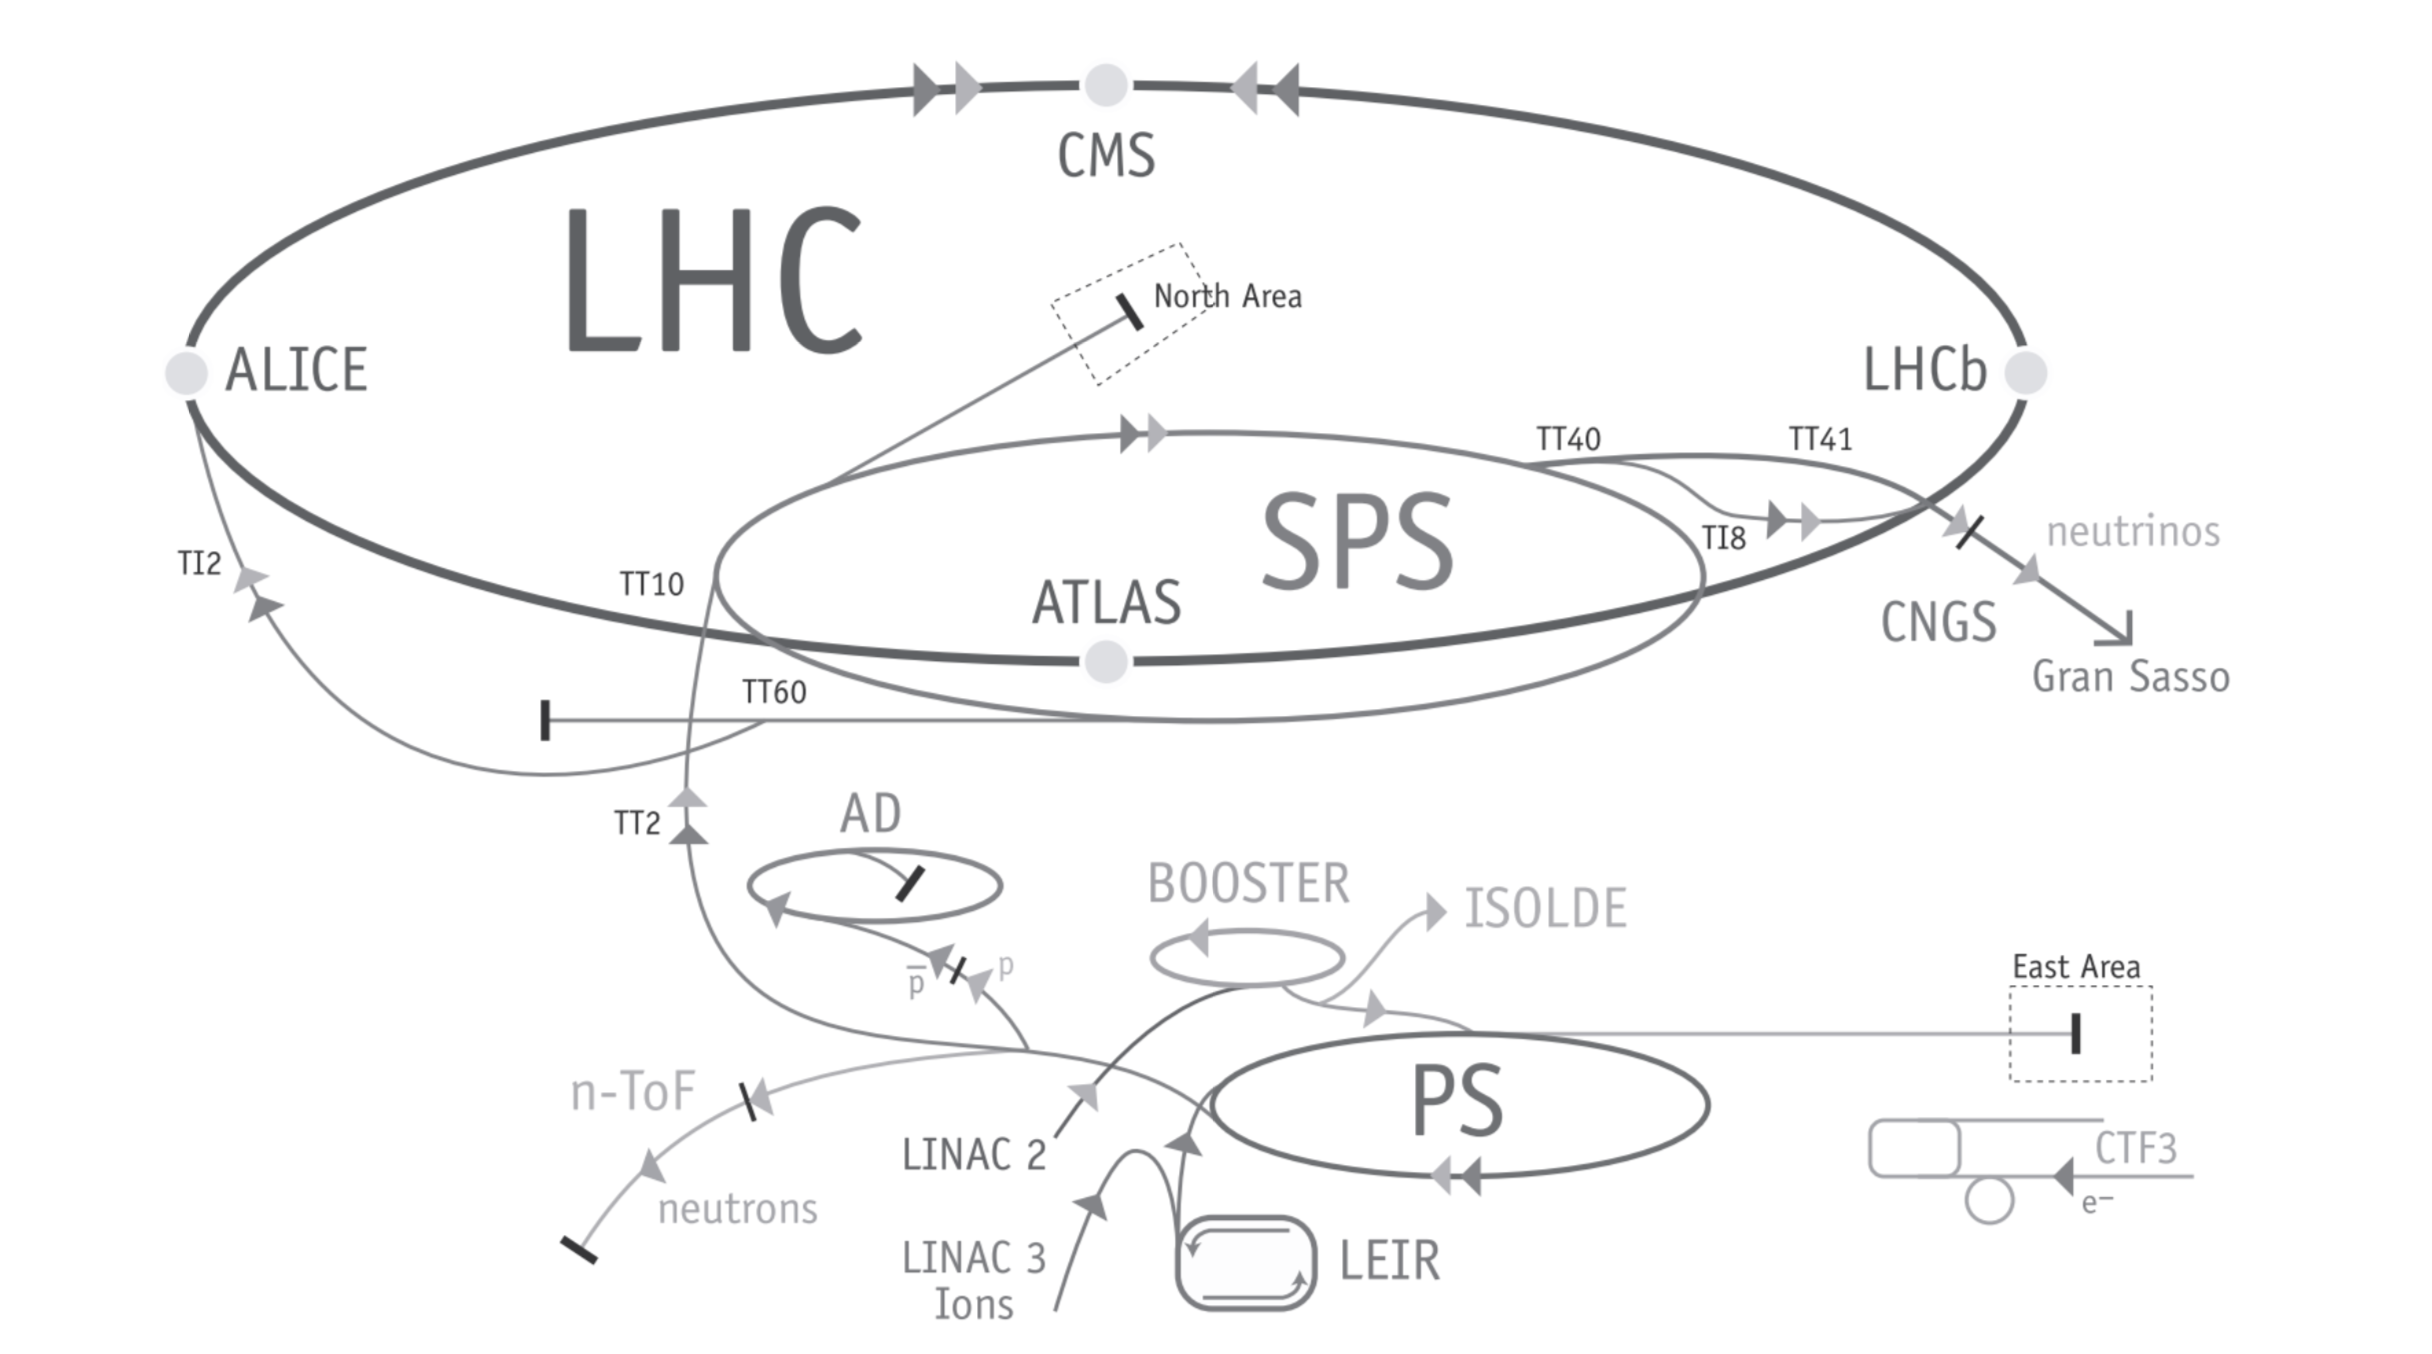
\includegraphics[width=0.7\linewidth]{Figures/LHC_struct}
	\caption{Schematic view of CERN's accelerator structure \parencite{CERN-Guide}}
	\label{fig:lhcstruct}
\end{figure}\\
As one can also see in this figure, there are four primary experiments and detectors situated in the acceleration ring. ALICE is a detector built for heavy ion collisions, LHCb is suitable for measuring top-quarks, ATLAS and CMS are both general purpose detectors. In the following section, the latter is going be introduced briefly, its measurements standing in the focus of this thesis.
\section{The CMS Detector}
The Compact Muon Solenoid (CMS) is a \SI{15}{\meter} wide and \SI{28.7}{\meter} long, onion-like-structured detector, consisting of five main components which are indicated in Fig.~\ref{fig:cms}.
\begin{figure}[h]
	\centering
	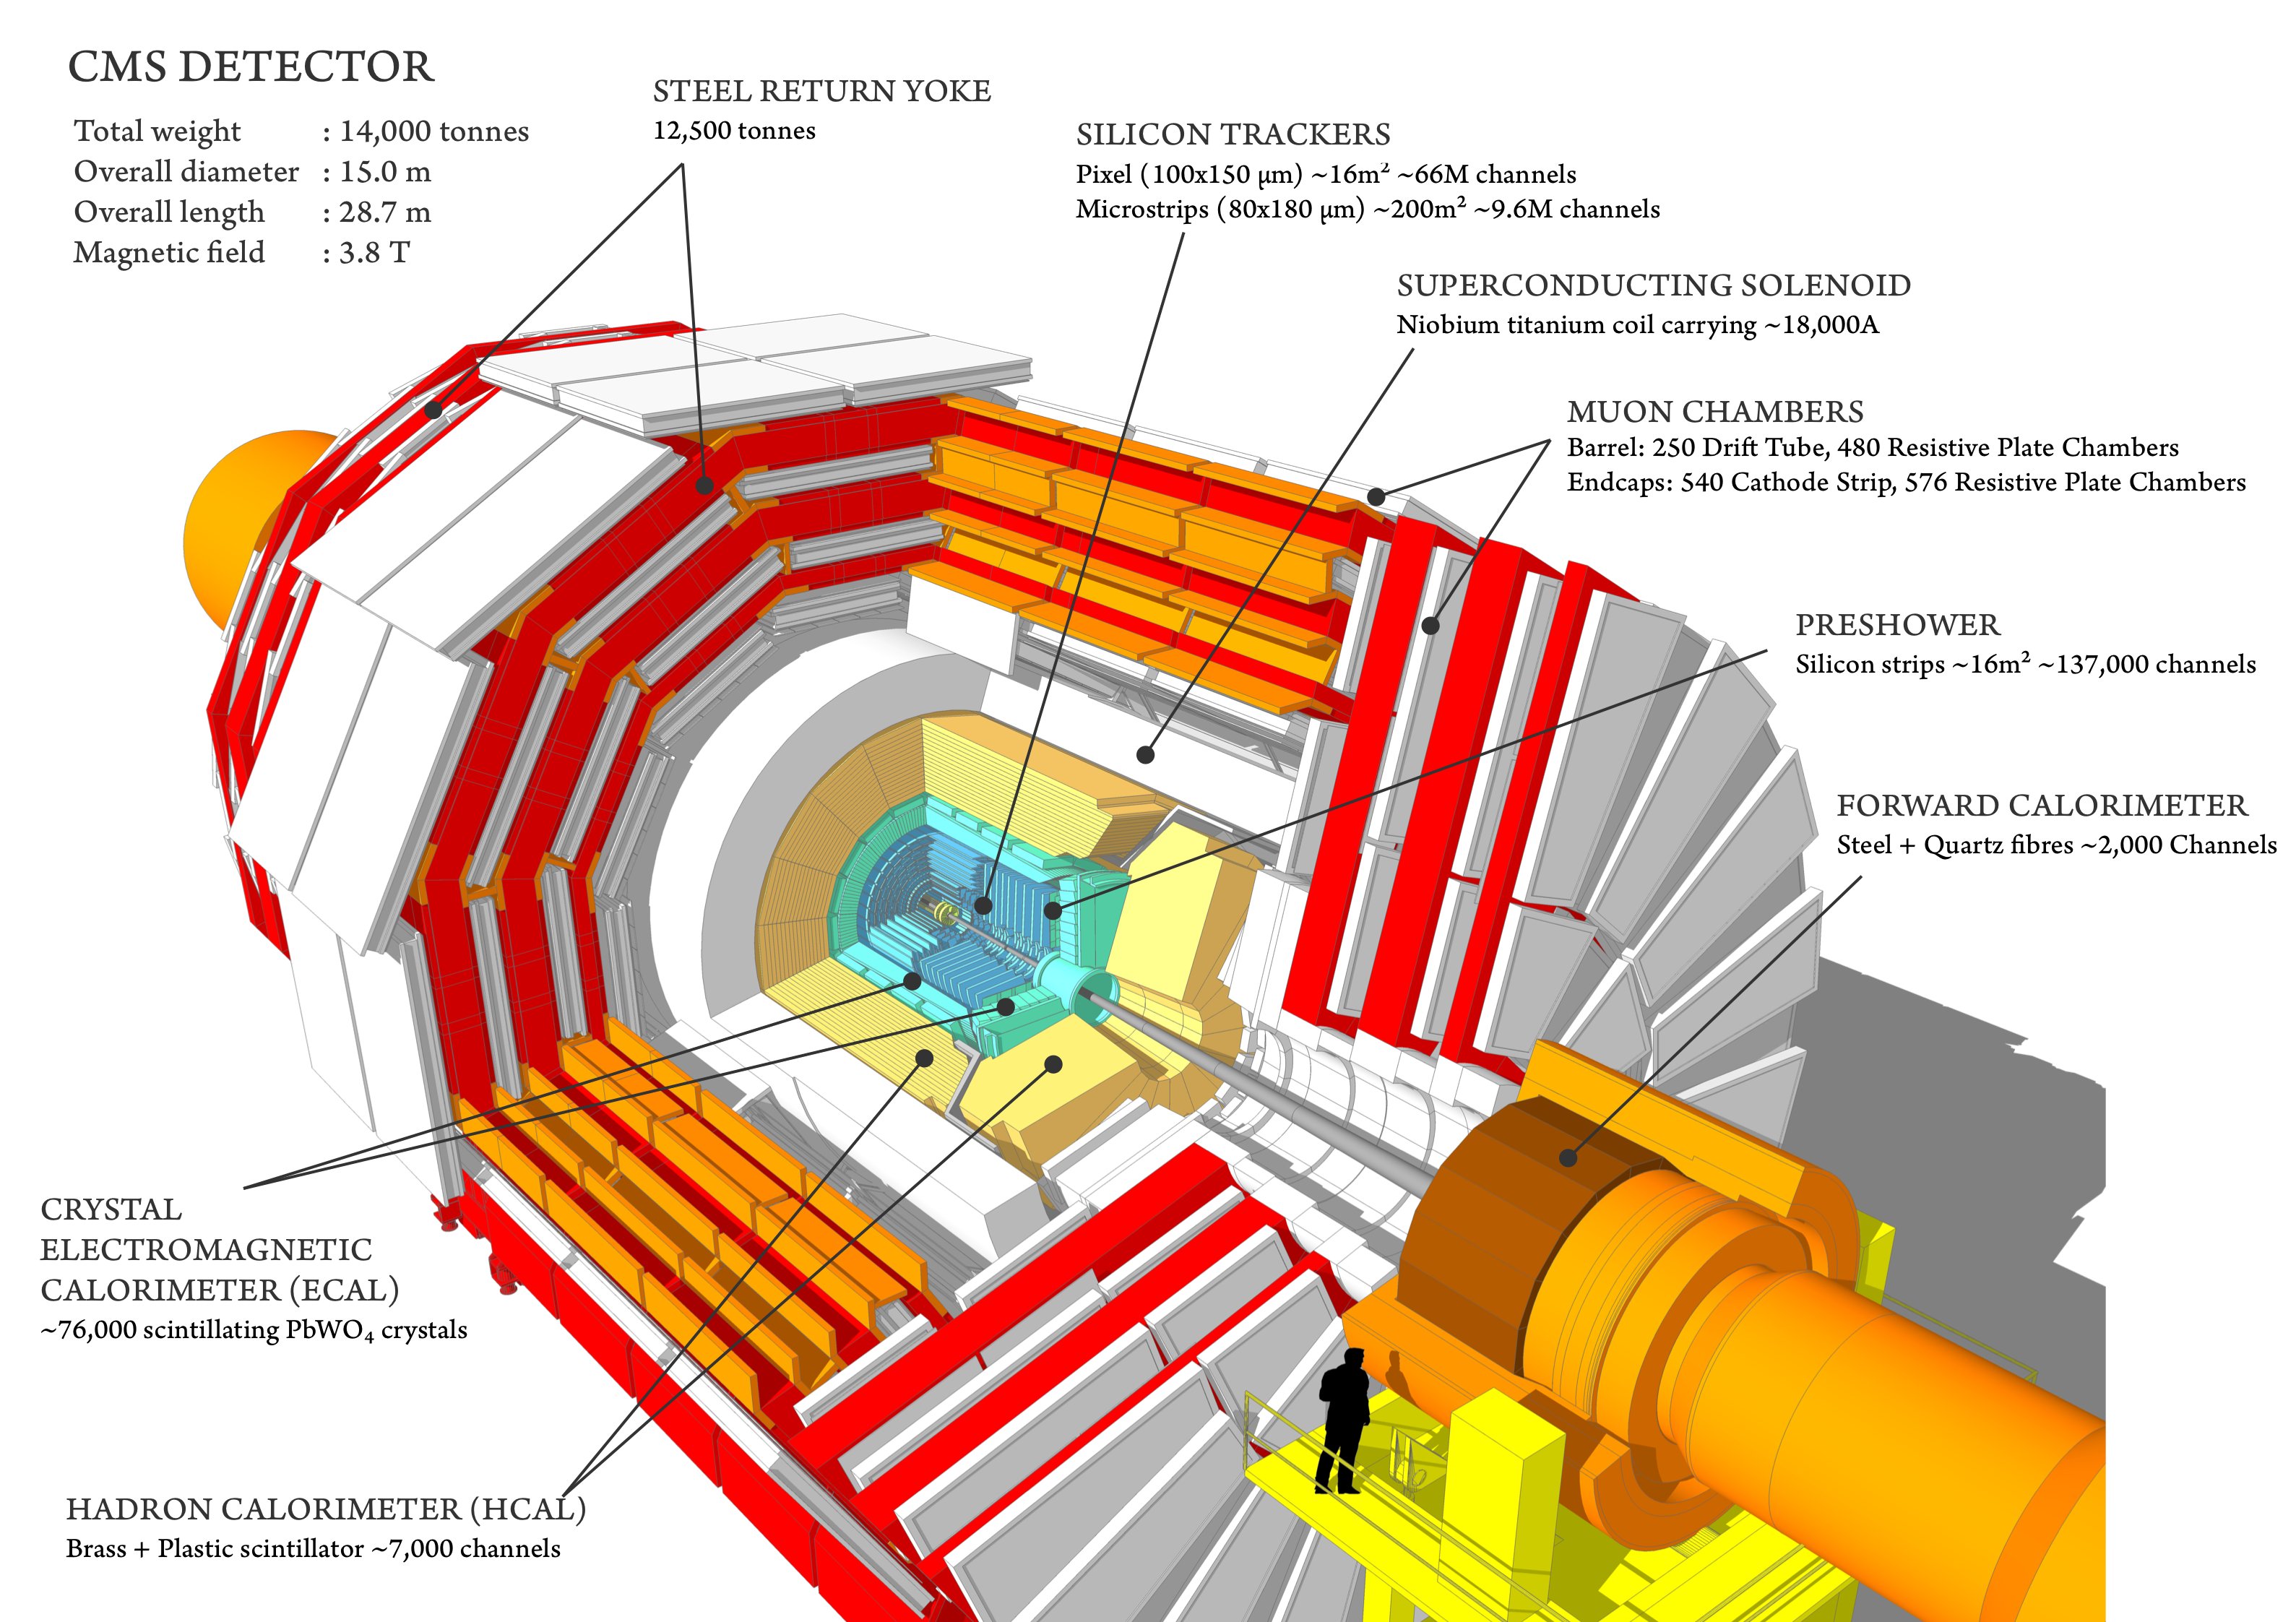
\includegraphics[width=0.9\linewidth]{Figures/CMS}
	\caption{The schematical structure of the CMS detector \parencite{CMS_Detector}}
	\label{fig:cms}
\end{figure}\\
It is built around a huge superconducting solenoid, which can generate a magnetic field of around \SI{3.8}{\tesla}. Its innermost detector component close to the interaction point (the spacial point where the particles collide) is a three layered silicon pixel detector, which with a resolution of 15-\SI{20}{\micro\meter} is capable of reconstructing impact parameters (which have a length of some
\SI{100}{\micro\meter}) and primary vertices. Around it, a silicon strip detector is situated, which can measure the trajectories of particles. Silicon was chosen due to the harsh environment around the collision point to increase the detector lifespan. With an active surface of \SI{200}{\meter\squared}, it is the largest silicon tracker ever built \parencite{CMS_collaboration}.\\
The second component is an electromagnetic calorimeter (ECAL) surrounding the silicon components, providing the measurement of the total energy of electrons and photons. These particles create electromagnetic showers, which can be converted into scintillator light by using lead tungstate crystals $\text{PbWO}_4$. Losing energy, the electrons and photons passing through the detector are eventually stopped in this component, delivering information about their total energy before entrance.\\
Surrounding the ECAL, the third component is the hadronic calorimeter (HCAL), capable of measuring the energy of hadronic jets. Consisting of brass and plastic scintillators, it functions similarly as the ECAL, as hadrons create a cascade of hadronic particles, generating light through scintillation.\\
The CMS detector is structured around the solenoid mentioned above. It is responsible for creating a strong and homogeneous magnetic field inside and outside of the coil in beam direction. This forces the particles to move along helical trajectories, from which through its radius the momentum of these can be measured in the tracking subdetectors.\\
Outside of the coil, the iron return yoke guides the magnetic field having a strength of around \SI{2}{\tesla}. Since muons are not stopped in the ECAL, this enables measuring their momentum for a second time, yielding better resolution and identification.\\
Since this thesis is centered around the measurement of impact parameters, the focus is going to be on the inner part of the detector, where the trajectories of the decay products can be measured.